\documentclass[../main/main.tex]{subfiles}


\begin{document}

\section{February 19th, 2021}
\subsection{Erikson's Psychosocial Theory}
\index{Erikson's psychosocial theory}
According to Erikson, development is determined by internal drives and social/cultural demands. On the one hand, we have our own demands, which may be unconscious , and on the other is put onto us by external factors.

Erikson also believes that there are 8 stages of development that everyone goes through, and for each, we must resolve some crisis or else we might not develop healthily. In addition, the stages are interconnected, meaning that the development of one stage might influence the development of another. Figure \ref{2-19-social} shows these 8 stages.

\begin{figure}[htpb]
  \centering
  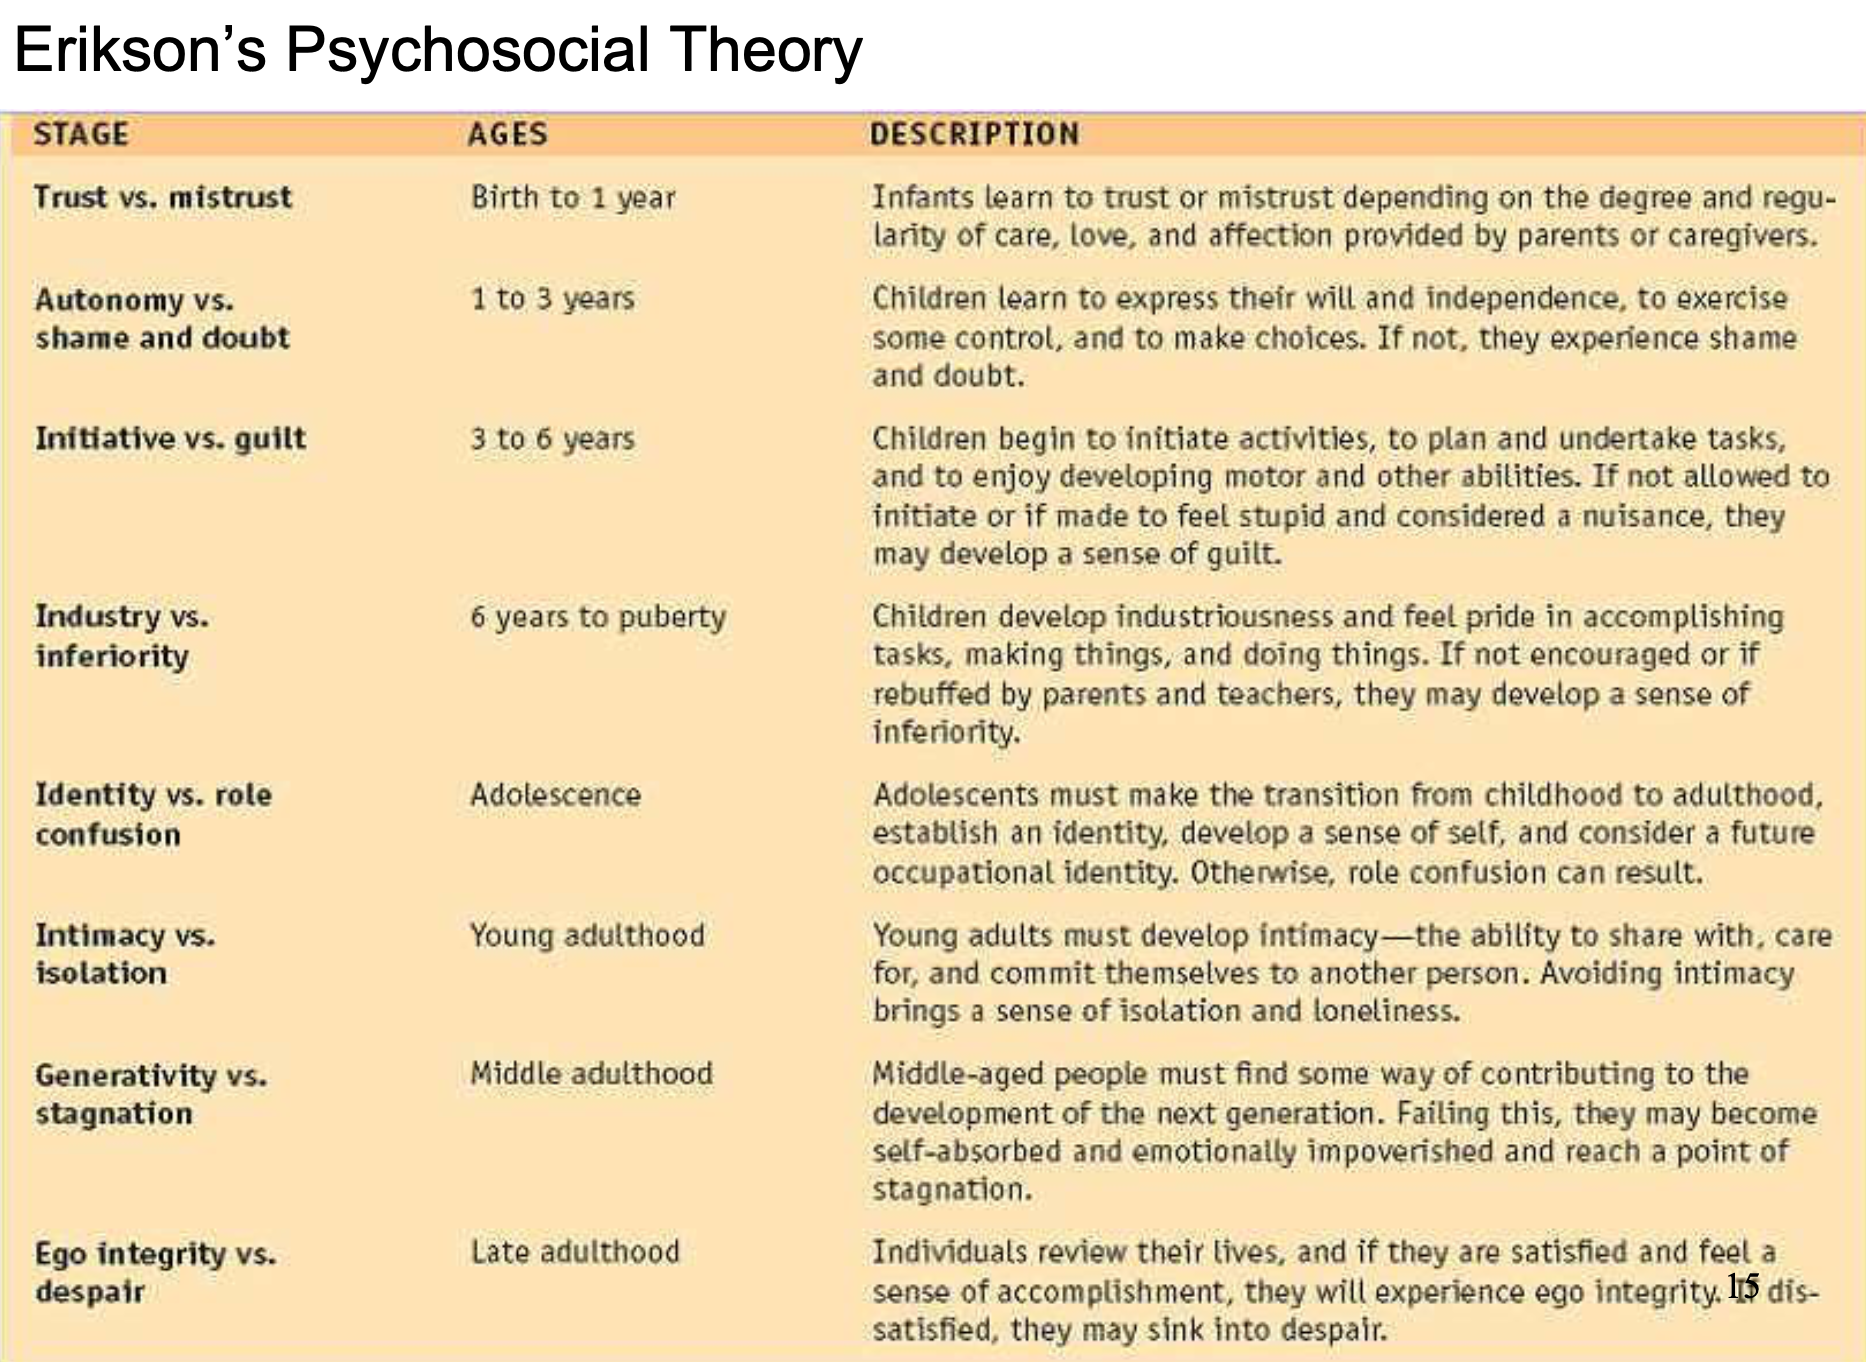
\includegraphics[width=\textwidth]{2-19-soc}
  \caption{Erikson's Psychosocial Theory}
  \label{2-19-social}
\end{figure}
\begin{description}
  \item[Trust vs. Mistrust (Birth - 1 year):] In the first stage, the infant learns to trust or mistrust the parent/caregiver.
  \item[Autonomy vs. Shame and Doubt (1-3 years):] In the second stage, the child wants to take control of things, e.g. which clothes to pick. If the parent provides them with this autonomy, then the child can develop the sense of autonomy. However, they must also set some boundaries
        \begin{remark}
According to Erikson, having a controlling parent is not healthy for the child's development. If they aren't provided with this autonomy, then the child will develop shame and doubt.
        \end{remark}
        \item[Initiate vs. Guilt (3-6 years):] In this stage, the child would like to initiate activities or make plans. If parents do not allow this, then the child will experience guilt.
        \begin{example}
The child might want to plan their own birthday.
        \end{example}
        \begin{remark}
This third stage is kind of like an extension of the previous stage.
        \end{remark}
    \item[Industry vs. Inferiority (6 years - pubery):] The child would like to feel pride in accomplishing tasks, making things, and doing things.
    \item[Identity vs. Role Confusion (adolescence):] The adolescents needs to establish an identity, and develop a sense of self, e.g. deciding what they want to do in the future, gender identity.
    \item[Intimacy vs. Isolation (young adulthood):] Young adults must develop intimacy, the ability ot share with,care for, and commit themselves to another person. Otherwise, the young adult would develop a sense of isolation and loneliness.
    \item[Generativity vs. Stagnation (middle adulthood):] The middle-aged person would like to find a way to contribute the next generation, e.g. having children or teaching others.
    \item[Ego integrity vs. Despair (late adulthood):] The person reviews their lives, and if they are satisfied, they will feel accomplished. Otherwise, they might sink into dispair.
\end{description}
\begin{remark}
Depending on whether we have more positive experiences than negative, we would have a better, more healthy development.
\end{remark}
% \begin{remark}
%   Even if we aren't able to resolve one stage, we will continue to the next one at the next stage of life.
% \end{remark}
\begin{remark}
  According to Erikson, even if we aren't able to resolve a crisis at a previous stage, we might be able to rectify it later. This is different from Freud's theory, which is more permanent.
\end{remark}
\begin{example}
Say the child's parent isn't very affectionate, and thus the child develops a mistrust in stage one. Later on, they might have positive experiences with others, e.g. a healthy long-term relationship. From these experiences, we can rectify it and develop trust in others.
\end{example}
\subsection{Discussion About Erikson's Theory}
Do you agree with Erikson's theory? Some comments from the class:

\begin{example}
  I disagree with Erikson’s theory:
  \begin{enumerate}
    \item I believe that development is more like a continuum which one learns and develop across time in different orders and timeframes, setting definite ranges in terms of age ignores individual differences;
\item Values and self-perception could be greatly affected by the environments around oneself - For instance, \textbf{there could be people who don’t feel that passing on to the next generation is necessary}
  \end{enumerate}
\end{example}
\begin{example}
I agree with the Erikson's theory. There are different needs in different stages of life. \textbf{However, there maybe overlapping for each area}. E.g. we build our industry (e.g. having good grades) and identity at the same time (e.g. bring a good student)\end{example}
\begin{example}
I also think that the pairs of adjective are \textbf{not really going in opposite directions} and not much logical explanation into why failing in one stage (e.g. in generatively vs stagnation leads to the feeling of stagnation)
\end{example}
\begin{example}
I think this theory ignore the factor of intrinsic traits of individuals (i.e. personality). Some may born to mistrust others regardless of their experiences. (\textbf{individual predispositions are ignored})
\end{example}
\begin{remark}[Summary of Discussion]
  \begin{itemize}
    \item Some crisis aren't fixed at a particular point in time, or might experience multiple at the same time
    \item Environment might be more important
    \item Some people might not experience a crisis at all (not applicable to everyone)
          \item The sequence of what crisis you experience might be different
  \end{itemize}
\end{remark}
\subsection{Evaluation of Erikson's Theory}
\begin{description}
  \item[Contributions:] Development is lifelong with changing needs (in contrast with Freud).
  \item[Limitations:]
        \begin{itemize}
          \item Not all individuals go through the same sequence
                \begin{example}
Some people might experience the crisis of intimacy before self-identity. They might find who they are through the relationship.
                \end{example}
                \item Oversimplifies development, as there is only one crisis in each period.
        \end{itemize}
\end{description}
\subsection{Behavioral Perspective} \index{behavioral perspective}
The previous theories were looking at development from the psychodynamic perspective. This section will cover the \vocab{behavioral perspective}, which says that development is shaped by the person's experience, such as environmental experiences or their upbringing.

According to psychologists who support the behavioral perspective, nurture is much more influential then nature.
\begin{definition}
According to the behavioral perspective, \vocab{learning} is a relatively permanent change in behavior (or behavioral capacity) brought about by \textbf{experience}. \index{learning}
\end{definition}
\subsubsection{Pavlov's Classical Conditioning Theory}
\index{Pavlov's classical conditioning theory}
Pavlov believe that all are actions are reactions to stimulus. Thus, \vocab{classical conditioning} is the type of learning in which a neutral stimulus comes to bring about a response after it is paired with a stimulus that naturally brings about that response.
\begin{definition} \index{neutral stimulus}
A \vocab{neutral stimulus} is a stimulus that does not bring a response in you.
\end{definition}
When we develop a reaction to a neutral stimulus, then we say that learning has occured. Pavlov's dog experiment is a famous example of this:
\begin{itemize}
  \item Initially the sound of the bell is neutral stimulus, meaning they don't naturally bring about a response.
\item Then meat, an unconditioned stimulus, is presented, which provokes a unconditioned response in the dog (salivation).
        \begin{definition} \index{unconditioned stimulus}
An \vocab{unconditioned stimulus} is a stimulus that naturally brings about a particular response without having been learned
        \end{definition} \index{unconditioned response}
        \begin{definition} An \vocab{unconditioned response} is a natural, reflexive response that needs no training
        \end{definition}
        \item During conditioning, the neutral stimulus is presented with the unconditioned stimulus, which triggers the response in the dog.
        \item After repeated exposure to this paring, the sound of the bell will trigger the response, thus making the sound of the bell a \vocab{conditioned stimulus (CS)} which triggers a \vocab{conditioned response (CR)}.
\end{itemize}

\begin{figure}[htpb]
  \centering
  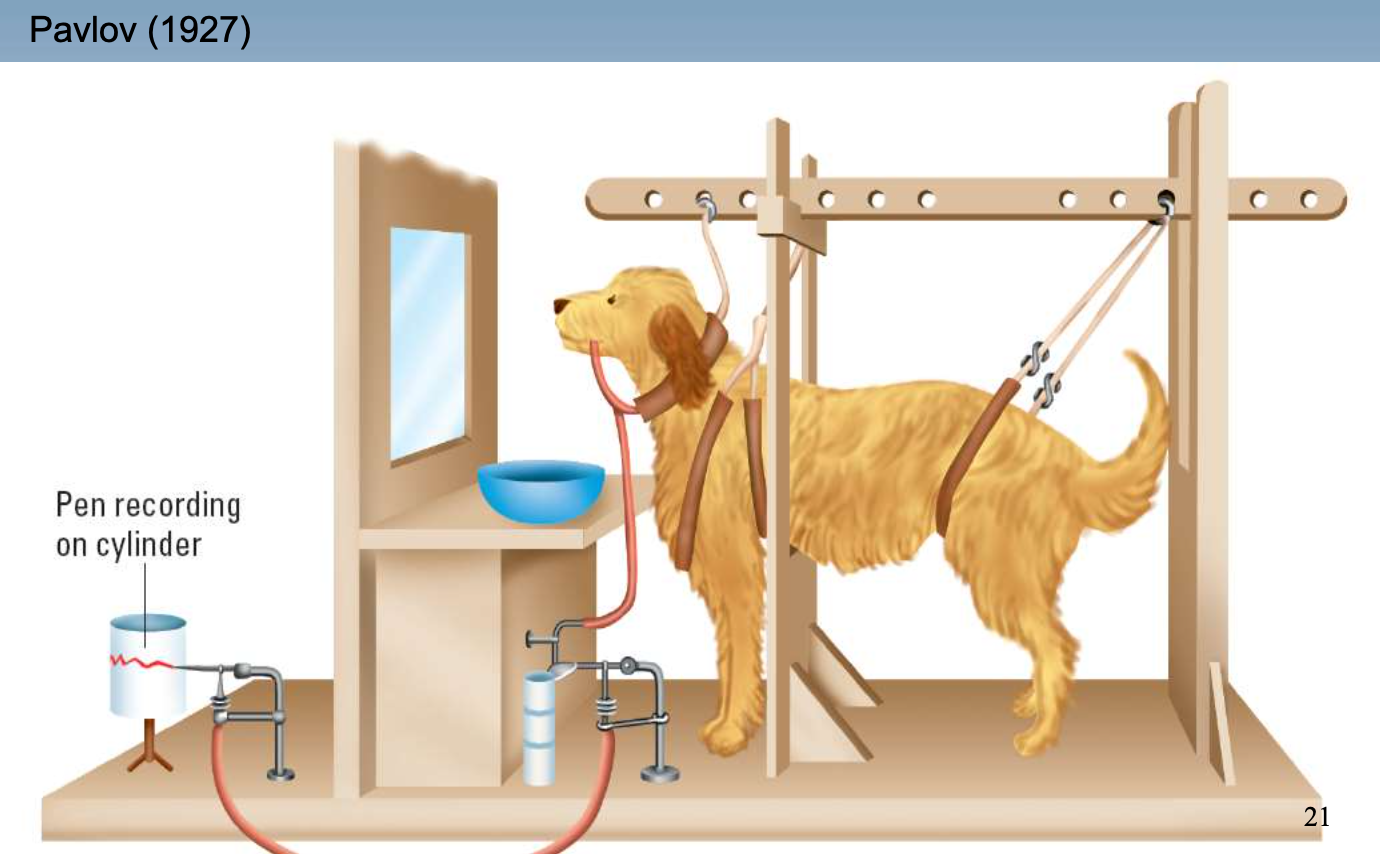
\includegraphics[width=0.8\textwidth]{2-19-pav}
  \caption{Pavlov's Conditioning Theory}
  \label{2-19-pav}
\end{figure}

\begin{remark}
  The conditioning process can be unlearned, after the dog realizes that the bell does not result in food.
\end{remark}
\begin{remark}
The timing between the stimulus presentation is important. Ideally, the neutral stimulus could be presented just before the unconditioned stimulus. Otherwise it won't be effective.
\end{remark}

The classical theory can explain how fear is developed in people. This can be seen in the ``Little Albert'' experiment (Watson, 1927):
\begin{itemize}
  \item Little Albert is not afraid of the rat and other things.
  \item Watson presents the rat with a clanging noise.
        \item Eventually, Little Albert is afraid, not just of the rat, but also of all furry things.
\end{itemize}
In this Little Albert experiment, we have the following:
\begin{description}
  \item[CS:] Rats/things white and furry
  \item[UCS:] Loud clang sound
  \item[CR/UCR:] Fear
\end{description}
\begin{remark}
Watson calls this \vocab{behaviorism}.
\end{remark}
\begin{figure}[htpb]
  \centering
  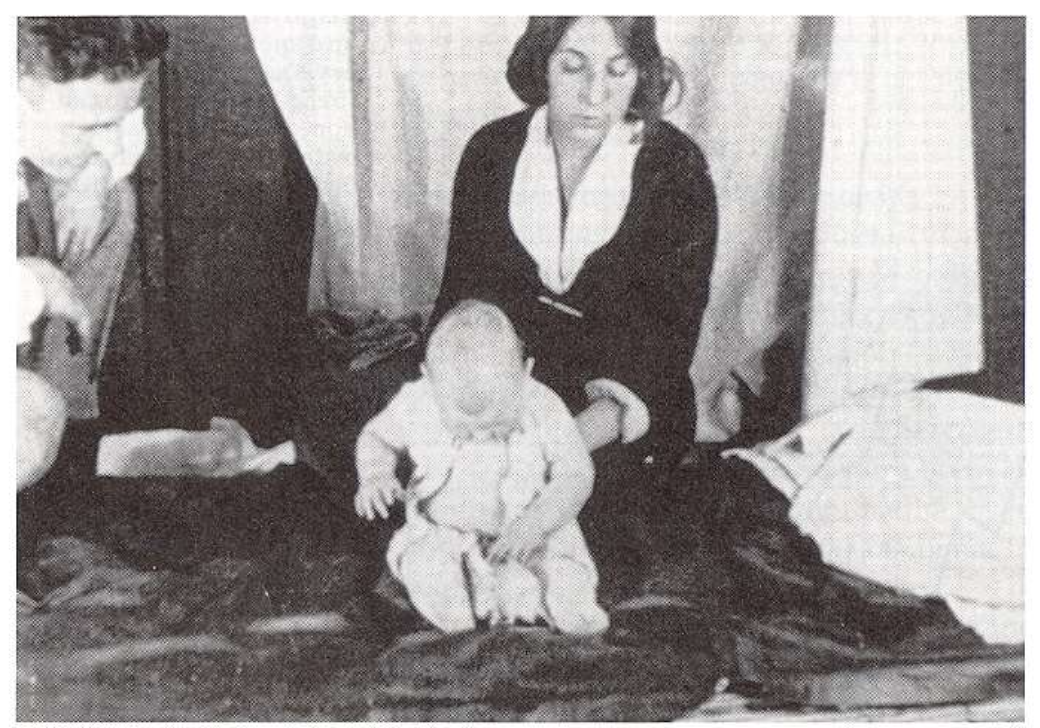
\includegraphics[width=0.8\textwidth]{2-19-alb}
  \caption{Little Albert was conditioned to fear rats}
  \label{2-19-alb}
\end{figure}

% \subsubsection{Skinner's Operant Conditioning Theory}
% \index{Skinner's operant conditioning theory}
% \subsubsection{Bandura's Social Cognitive Theory}
% \index{Bandura's social cognititve theory}






\end{document}
